\documentclass[10pt,a4paper]{article}
\usepackage[utf8]{inputenc}
\usepackage{amsmath}
\usepackage{amsfonts}
\usepackage{amssymb}
\usepackage{hyperref}
\usepackage{listings}
\usepackage[many]{tcolorbox}
\tcbuselibrary{listings}

\newtcblisting{mylisting}{
  listing only,
  hbox,
  colframe=cyan,
  colback=cyan!10,
  listing options={
    basicstyle=\small\ttfamily,
    breaklines=true,
    columns=fullflexible
  },
}

%hyperlink parameters
\hypersetup{
    colorlinks=true,
    linkcolor=blue,
    filecolor=magenta,      
    urlcolor=cyan,
    pdftitle={Overleaf Example},
    pdfpagemode=FullScreen,
    }
\urlstyle{same}

\author{Sarah}
\title{OpenACC using Colab}
%\date{today}

\begin{document}
\maketitle{}
\newpage

\section{Part 1: Introduction}
This document offers an introduction to porting algorithms on GPU with OpenACC using Colab.\\

\section{Part 2: Running a Fortran code in Colab}
\subsection{About Colab}
Colab is a free cloud service proposed by Google based on the Web Open Source application Jupyter-Notebook.


\subsubsection{Compilation and Execution}
Here, we use the tutorial proposed by \href{https://colab.research.google.com/github/ENCCS/OpenACC-CUDA-beginners/blob/colab_gcc/examples/openACC_CUDA_colab.ipynb#scrollTo=6WS9YBwSAsnf}{}

\subsubsection{Preview on the CPU code}
Before thinking about optimizing an application, one should first make a performance-profiling and find hotspots in the source code. In other words, the idea is to get information about.\\
Let's note that in Fortran language, considering a two dimensions array, the reading is made column by line. 

\subsubsection{OpenACC}
Most of what will be presented here comes from this \href{https://colab.research.google.com/github/ENCCS/OpenACC-CUDA-beginners/blob/colab_gcc/examples/openACC_CUDA_colab.ipynb}{tutorial}.\\
OpenACC is a directive-base programming approach.
\begin{lstlisting}
!nvidia-smi
\end{lstlisting}
Here the outcome of this command:
\begin{center}
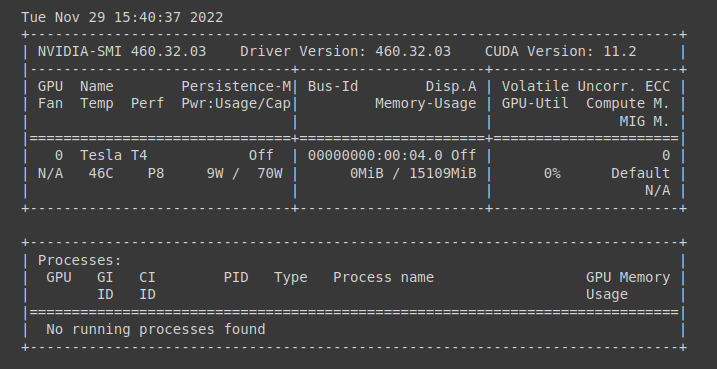
\includegraphics[scale=0.8]{nvidiasmi.png}
\end{center}

\subsubsection{GPU Runtime}
Enable GPU in the file.

\end{document}